\section{Finance Simulation}
\label{sec:finance_simulation}

\subsection{The Finance Graph}
%nike, salih
The finance simulation is connected to almost all other simulations, as costs and profits are ruling an enterprise's daily work. The complete finance graph can be found in appendix \ref{fig:finance_graph}, however, it is part of the overall graph. Just for reasons of clarification and concise structure we developed a separate graph, whereas at least the start node and the leave nodes are exactly the same as in the overall graph. Contrary to the overall graph, we inserted aggregated nodes, that simply sum up the nodes in the overall graphs, for a clearer overview about how the single financial performance indicators are calculated. Especially for the calculation of the \gls{EBIT} this graph is important, because it displays all the expenses and all the revenues from different sources neat and clean. These aggregated total nodes are:
\begin{itemize}
    \item \textit{totalMarketingCosts (tMC)}
    \item \textit{totalLogisticCosts (tLC)}
    \item \textit{totalHRCosts (tHRC)}
    \item \textit{totalSupportCosts (tSC)}
    \item \textit{totalWarehouseCosts (tWH)}
    \item \textit{totalProductCosts (tPC)}
    \item \textit{totalRevenues}
\end{itemize}

\subsection{Calculation of Financial Key Figures}
\subsubsection{Company Net Worth}
The main financial key figure is the company net worth (\textit{netWorth}). A company's net worth is the difference between assets and liabilities\footnote{https://www.investopedia.com/terms/n/networth.asp}. In a successful company, this value should be positive and increase continuously. This is adapted from a balance sheet that is usually updated annually. The balance sheet template in table \ref{tab:balanceSheet} shows an exemplary balance sheet in CapitalismX which is updated daily for the calculations in the backend. On the assets side there are non-current assets, which include buildings, machinery, vehicle fleets and investments, and current assets, which include components, products, bank and cash. On the liabilities side, the equity capital and the liabilities are shown including loans and total expenses.

However, in CapitalismX the company \textit{netWorth} as well as all other financial key figures are calculated in a simplified manner, due to the high complexity in the real world. The company \textit{netWorth} is calculated in equation \ref{func:netWorth}. Currently, the player gets 1,000,000 CapCoins equity capital as starting capital. In later implementation, this value needs to be adjusted according to tests with all financial costs and profits. Also, currently the balance sheet in the prototype does neither include the current assets nor the total expenses, due to reasons of complexity. Nevertheless, the current assets as well as the total expenses are included in the operations section of the finance dashboard, which is explained in section \ref{sec:finance_dashboard}.

\begin{table}[ht]
\begin{tabular}{|p{5.8cm}|p{5.8cm}|}
\hline
\multicolumn{2}{|c|}{\textbf{Balance Sheet}}\\
\hline \textbf{Assets} & \textbf{Liabilities}\\ 
\hline \textbf{I. Non-current assets} & \textbf{I. Equity capital}\\
\hline 1.2 Land and buildings &\\
\hline 1.3 Machines & \textbf{II. Liabilities}\\
\hline 1.4 Vehicle fleet & 2.1 Loans\\
\hline 1.5. Financial investments &  2.2 Total expenses\\
\hline &\\
\hline \textbf{II. Current assets} &\\
\hline 2.1 Components &\\
\hline 2.2 Products &\\
\hline 2.3 Bank and cash &\\
\hline &\\
\hline \textbf{Total Assets} & \textbf{Total Liabilities}\\
\hline
\end{tabular}
\caption{Balance Sheet}
\label{tab:balanceSheet}
\end{table}

\begin{equation}
\label{func:netWorth}
\begin{split}
    netWorth = cash + assets - liabilities \\ ~\text{whereas}~liabilities = loanAmount
    \end{split}
\end{equation}

\subsubsection{The Relation Between Assets and Cash}

The company's assets are defined as the sum of fleet (\textit{totalTruckValues}), equipment for production (\textit{totalMachineValues}), value of buildings (\textit{totalWarehousingValues}), and the investments earned (\textit{totalInvestmentAmount}), which is displayed in equation \ref{func:assets}:
\begin{equation}
    \label{func:assets}
    \begin{aligned}
        assets = & ~totalTruckValues \\
        &+ totalMachineValues \\ 
        &+ totalWarehousingValues \\
        &+ totalInvestmentAmount
    \end{aligned}
\end{equation}

The cash can be calculated as follows in equation \ref{func:cash}, whereas the current cash amount, which is calculated on a daily basis, is added to the former amount of cash. This is displayed by $+=$ which is the addition assignment operator.
\begin{equation}
    \label{func:cash}
    cash \mathrel{+}= NOPAT + assetsSold 
\end{equation}

% Describe relationship between assets and cash, so if buying a machine is shoving money from cash to assets
When purchasing assets, the amount of the asset's \textit{purchasePrice} is simply shoved from cash to assets, because the value of assets increases whereas the cash decreases by the amount of the \textit{purchasePrice}. This accounting exchange does not affect the \textit{netWorth}.
The assets of a company consist of elements necessary to operate productively. The \textit{purchasePrice} of an asset is reported in the balance sheet in order to identify impairment. In CapitalismX, this is represented by a straight-line depreciation using the formula \ref{calc:depreciation}. 
    
\begin{equation}
     \label{calc:depreciation}
     Annual \ depreciation = {\frac{purchasePrice}{useful \ life \ of \ the \ asset}}
\end{equation}
If the player now decides to sell one of the assets before the end of its useful life, he can sell it at its residual value, which is the \textit{resellPrice} (\ref{calc:residualvalue}). 
\begin{equation}
     \label{calc:residualvalue}
     resellPrice = {{purchasePrice} - {annual \ depreciation \cdot t }}
\end{equation}

If assets are sold, the \textit{cash} increases by the amount of \textit{assetsSold}, which are defined by the following values:
   
\begin{itemize}
    \item \textit{totalWarehouseValues}. The player has the possibility to build a warehouse to store his products. However, it may happen that the warehouse is no longer needed. 
    The cost calculation of the warehouse and the useful life are described in chapter \ref{warehouse_simulation}. The sum of all resold warehouses is described by the \textit{totalWarehouseValues}, 
    \begin{equation}
        totalWarehouseValues = \sum resellPrice_{Warehouse}
    \end{equation}
    \item \textit{totalTruckValues}. Similar to the resale of buildings it is also possible to sell the vehicles at their residual value if they are no longer used or the delivery is carried out by a logistics partner. The cost of the vehicles and their useful life are described in Chapter \ref{logistic_simulation}.
    \begin{equation}
        totalTruckValues = \sum resellPrice_{Truck}
    \end{equation}
    \item \textit{totalMachineValues}. The player has the possibility to sell used machinery, that he or she does not need anymore. The calculation for the residual value is based on a modified depreciation because our machinery can be maintained or upgraded. The calculation can be found in chapter \ref{sec:productionSim}. The \textit{resellPrice} corresponds to the equation \ref{eq:sellMachine}.
    \begin{equation}
        totalMachineValues = \sum resellPrice_{Machinery}
    \end{equation}
\end{itemize}

Also investments decrease cash and increase assets when bought. Investment returns are either positive or negative incomes from the investment area in the financial dashboard. Investing in real estate funds, stocks or venture capital can provide the player with an investment gain, which is displayed in the finance view \ref{fig:finance_view}. However, if he risks too much, he can suffer high losses and thus put his own company at risk. Chapter \ref{sec:investments_simulation} describes the process in detail.

\subsubsection{NOPAT}

The next important key figure is the \gls{NOPAT}. The \textit{NOPAT} can be calculated by subtracting the \textit{incomeTax} and the \textit{interestsLoan} from the \textit{EBIT}. The \gls{EBIT} is the amount of money, that the player has obtained through his or her actions during the game. The calculation of the \textit{NOPAT} can be found in equation \ref{func:NOPAT}.
\begin{equation}
    \label{func:NOPAT}
    NOPAT = EBIT - incomeTax - interestLoan 
\end{equation}
 
\subsubsection{Income tax}
\label{sec:incomeTax}

In CapitalismX the \textit{incomeTax} is levied on a daily basis and can be compared to the income tax paid by a large corporation in the United States of America according to the IAS 12 \textit{Income Taxes} paragraph from the IFRS\footnote{https://www.ifrs.org/-/media/feature/meetings/2018/october/iasb/ap12c-ias12.pdf}. To determine realistic tax rates, corporations selling similar products to the ones in CapitalismX were compared, using the IFRS statements from yahoo finance, resulting is a \textit{taxRate} of 20\% for CapitalismX. The compared corporations with their tax rate can be seen in table \ref{Example_Tax}.

\begin{table}[!h]
\centering
\begin{tabular}{|l|l|l|l|l|l|l|}
\hline
Example & IBM & HP Enterprise & Google & Nintendo & Apple & Average \\
Tax Rate & 23\% & 16\% & 12\% & 30\% & 18\% & 20\% \\ \hline
\end{tabular}
\caption{Example Tax rates}
\label{Example_Tax}
\end{table}

Realistically the income tax is levied annually, but in order to provide the player a more structured overview about the company’s financial situation, we decided to provide the player with a daily \textit{incomeTax}, as calculated in equation \ref{func:incomeTax}. 
\begin{equation}
    \label{func:incomeTax}
    incomeTax = EBIT \cdot taxRate
\end{equation}

As described in chapter \ref{logistic_simulation} the produced products per day are collected in the warehouse and sent out to the market at the end of the day. Hence, the amount of the \textit{incomeTax} varies depending on the quantity of products sold. Lobbyists, who can be hired, have a political influence on the \textit{taxRate}. This process is described in chapter \ref{lobbyist_simulation}.

\subsubsection{EBIT}

The next level under the company's \textit{NOPAT} is the \textit{EBIT}, which are the earnings before interest and tax, a commonly used key financial indicator in company's financial statements. \cite{lee_e_2006} Again, the calculation of the \textit{EBIT} is simplified for the business simulation game at hand. To sum it up, the revenues are added to the \textit{EBIT} whereas the total expenses are subtracted. The \textit{EBIT} is displayed in the operations section of the finance view and updated on a daily basis. This means, also the total revenues and total expenses are calculated on a daily basis.\\
\\
\textbf{Revenues}\\
\\
The total revenue is calculated by adding all incoming cash flows from the goods sold (\textit{productSale}). The sum of \textit{productSale} is displayed by the \textit{totalSalesRevenues}, which can be derived by multiplying a product’s sales price \textit{(sP)} with the amount of units sold, which are the sales figures (\gls{sFig}). 
    \begin{equation}
        totalSalesRevenue~(\gls{tSR}) = \sum_{p \in P}(sFig \cdot sP) 
    \end{equation}
To put it into a nutshell, the total revenues equal the \textit{totalSalesRevenue} calculated according to the equation \ref{func:totalRevenue}:

\begin{equation}
\label{func:totalRevenue}
    totalRevenues = ~totalSalesRevenues 
\end{equation}\\
\\
\textbf{Expenses}\\
\\
The other part needed to calculate the EBIT are the total expenses. All costs and expenditures that occur across all other simulations are accounted as expenses. The total expenses consist of:
\begin{itemize}
    \item \textit{totalHRCosts} (\textit{tHRC}), which is the sum of all salaries and the aggregated sum of all trainings and courses for employees. 
    \begin{equation}
        totalHRCosts~(\gls{tHRC}) = totalSalaries \ + \  totalTrainingCosts
    \end{equation}
    whereas all trainings (\gls{TR}) have a price, which is a property of the object \textit{trainings}.
    \begin{equation}
        totalTrainingCosts = \sum_{tr \in TR} tr.cost
    \end{equation}
    and all employees (\gls{E}) have a specific salary, which is a property of the object \textit{employee}.
     \begin{equation}
        totalSalaries = \sum_{e\in E} e.salary
    \end{equation}
    The calculation of these costs can be found in chapter \ref{sec:HRsim}.
    \item \textit{totalWarehouseCosts} (\textit{tWC}), which is the sum of the acquisition costs for all warehouses, the monthly costs for warehouses \textit{cWH} (cf. equation \ref{func:cWH}) and the daily storage costs \textit{sC} (cf. equation \ref{func:SC}). All produced goods are collected at a warehouse and sent out to the market at the end of the day but they do not cause storing costs. Only when producing more products than the market currently demands the spare products are stored in a warehouse, which causes warehousing and storage costs. Added to that, the components which are not manufactured into products yet generate warehousing costs, as they need to be stored until ready for production. 
    \begin{equation}
        totalWarehouseCosts~(tWC) = cWH + sC
    \end{equation}
    The calculation of the storing and the acquisition costs can be found in chapter \ref{warehouse_simulation}. 
    \item \textit{totalLogisticCost} (\textit{tLC}), which occur inevitably when selling or retailing goods. The total logistic costs depend on the type of logistics chosen by the player. There are three options: sending packages with an own internal fleet, outsource to an external logistics partner, and a combination of external partners and own fleet. The total logistic costs can be calculated as follows:
    \begin{equation} 
        totalLogisticCosts~(tLC) = cL + tDC
    \end{equation}
    The exact calculation of these costs can be found in chapter \ref{logistic_simulation}.
    \item \textit{totalProductCosts} (\textit{tPC}), which occur when manufacturing components to products. The calculation of these costs can be found in chapter \ref{sec:productionSim}. The total production costs is the sum of variable and fixed production costs.
   \begin{equation}
       totalProductionCosts~(tPC) = variableCosts_{perProduct} + fixedCosts
   \end{equation}
    \item \textit{totalMarketingCosts} (\textit{tMC}), which occur when starting marketing activities like marketing campaigns, market research or press releases (cf. chapter \ref{market_research_simulation}). The total marketing costs also include all costs that are derived from activities to improve the company image, such as hiring a management consultant, donating for social engagements, or promoting a green company image. These costs can be found in chapter \ref{company_image}. Also, hiring a lobbyist for political reasons or to decrease the tax percentage, belongs to the total marketing costs. The calculation of these costs can be found in chapter \ref{lobbyist_simulation}. Accordingly, the total marketing costs are aggregated as follows:
    \begin{equation}
    \begin{split}
        totalMarketingCosts~ (\gls{tMC}) = price_{managementConsultancy} \\
        + price_{marketResearch} \\
        + price_{campaign} \\
        + price_{lobbyist} \\
    \end{split}
    \end{equation}
    \item \textit{totalSupportCosts} (\textit{tSC}), which occur if the player chooses to offer product support and maintenance for customers. The \textit{tSC} calculation can be found in chapter \ref{product_support_simulation}.
\end{itemize}

According to the list of total revenues and total expenses above, the EBIT can be calculated as follows in function \ref{func:ebit1}. This equation is illustrated by the total finance graph, which can be found in the appendix \ref{fig:finance_graph}.  
\begin{equation}
\label{func:ebit1}
    EBIT = totalRevenues - totalExpenses
\end{equation}
whereas total revenues are calculated as in function \ref{func:totalRevenue}, and total expenses are calculated as in the following function \ref{func:ebit2}
\begin{equation}
    \label{func:ebit2}
    \begin{aligned}
       totalExpenses = tHRC + tWC + tLC + tPC + tMC + tSC
    \end{aligned}
\end{equation}

\subsection{Banking system}
\label{sec: banking}

The bank simulation ensures that the player has an additional opportunity to raise capital in case of bottlenecks or for investments. Three types of credit are offered to the player in case of a request \footnote{https://www.statista.com/statistics/258174/long-term-interest-rates-worldwide}. Table \ref{loan_types} lists the terms and interest rates for the different loan types. 

\begin{table}[ht]
\centering
\begin{tabular}{|l|r|r|}
\hline
loan Type       & interest rate (\textit{interestsLoan})     & duration \\ \hline
short-term      & 6-18\%           & 1-12 months    \\
medium-term     & 3-6\%            & 1-5 years     \\
long-term       & 1-3\%             & 10-15 years     \\
\hline
\end{tabular}
\caption{Interest Rate and Duration of loan Types}
\label{loan_types}
\end{table}

The bank's credit offers are randomized in the defined intervals to make the game more interesting for the player. Hence, both variables, the duration as well as the interest rates, are randomized on a daily basis. The three types of credit are provided as amortization loans. Thus, the player has a fixed interest rate and a fixed monthly amortization. This reduces the repayment amount over time \footnote{\footnote{https://www.investopedia.com/terms/a/amortized\_loan.asp}}.
After the player has entered the desired loan amount (defined by the variable \gls{S}), the bank checks the creditworthiness. Based on this, the three loan offers are calculated in the backend. To determine the term (\gls{t}), a random number is generated for each credit type . Thus, the annual repayment (\gls{a}) can be determined as follows \ref{func:repayment}:

\begin{equation}
\label{func:repayment}
\begin{aligned}
repayment (a)= {\dfrac{S}{t}}
\end{aligned}    
\end{equation}

Once the loan amount and term values have been determined, an interest rate (\gls{i}) per credit type is generated again randomly using the above intervals. To calculate an annual interest rate, the remaining principal balance per year (\textit{S\textsubscript{t}}) must first be calculated for each year. The remaining \textsubscript{t}  is the starting value at the beginning of the following year to calculate the interest rate per year (\textit{i\textsubscript{t}}). This results in the following formulas \ref{func:interestrate}:
\begin{equation}
\label{func:interestrate}
\begin{aligned}
principal \ balance \ per \ year (S\textsubscript{t})= S- (a \cdot t)\\
Interest \ rate \ per \ year (i\textsubscript{t}) = S\textsubscript{t} \cdot i
\end{aligned}    
\end{equation}

Thus, an annual rate is calculated in function \ref{func: rate}, which has to be paid by the player for the loan amount taken up.

\begin{equation}
\label{func: rate}
\begin{aligned}
loanRate = a+ i\textsubscript{t}
\end{aligned}    
\end{equation}

An exemplary repayment model for a midterm loan can be seen in the Appendix \ref{fig:loanRepayment} where all the above described equation are summed up in a table.
However, the raising of capital from the bank is restricted.
The requested loan \textit{S} must not be larger than 70 \% of the company value, which is for reasons of simplification the current company net worth. If this is fulfilled, the player receives three offers with the duration and the interest rate as described above. In the event of a negative check by the bank, so if the requested loan \textit{S} is in fact larger than 70\% of the company value, then the player receives an adjusted offer corresponding to the company value. The new loan amount offered is not greater than 70\% of the company value. The process of the banking simulation is displayed in an activity diagram in figure \ref{jpg:banking}.\\
For a better understanding, the following algorithm can be helpful:
\begin{equation}
    \begin{aligned}
         \texttt{If S} \leq \texttt{netWorth} \cdot 70\%  \xrightarrow{} \text{accept AND offer three credit forms} \\
         \texttt{If S} > \texttt{netWorth} \cdot 70\%  \xrightarrow{} \text{reject AND offer} \ (\texttt{netWorth} \cdot 70\%)
    \end{aligned}    
\end{equation}

\begin{figure} [h]
	\centering
	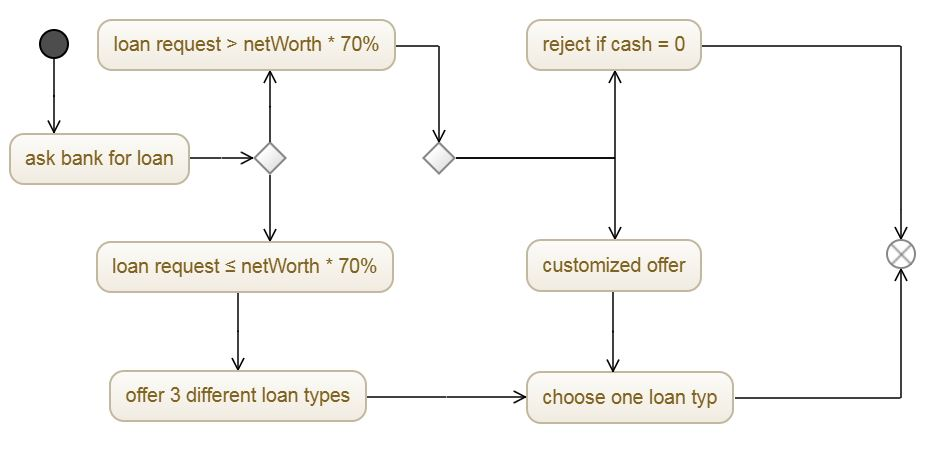
\includegraphics[width=12cm]{images/activity_diagram.JPG}
	\caption{Activity Diagram Banking Simulation}
	\label{jpg:banking}
\end{figure}


\subsection{Investments}
\label{sec:investments_simulation}

 Investments in CapitalismX are a way to allocate your residual cash to assets with an expected profit. However, each investment is risky and positive return isn't guaranteed. Thus, your liquidity may suffer if you put too much money into investments.
  
  We decided for three classes of investments with different expected returns and assume higher risk for higher return:
\begin{itemize}
	\item Real estate fund
	\item Stocks (index fund)
	\item Venture capital fund
\end{itemize}

Although return distributions are negatively skewed and characterized by an excess kurtosis \cite{ANDERSEN200143}, a normal distribution can be used as an approximation \cite{doi:10.1080/01621459.1972.10481297}. In 2017, the expected return for real estate in the US is about $7\%$ \footnote{https://www.msci.com/documents/10199/f3d1af7c-6069-6e60-a818-71ca9c45e85c}. The compounded annual return of the S\&P from its introduction in 1965 to 2017 is approximately $10\%$ \footnote{http://www.berkshirehathaway.com/letters/2017ltr.pdf}. Venture capital funds in the US have an expected return of $14.2\%$ \footnote{http://www.eif.org/news\_centre/publications/eif\_wp\_41.pdf}.

In our game, the investment worth adjusts daily. Therefore, we take the geometric mean of the average yearly return $\overline{\mu_y}$ to estimate the expected daily return:
\begin{equation}
	\overline{\mu_d} = \sqrt[365]{\frac{1 + \overline{\mu_y}}{1}}
\end{equation}

For our game, we use the return volatility as a representative of the risk of an investment. In an efficient market, a higher risk has to correspond to a higher return. As we are not able to model more complex anomalies like volatility clustering \cite{lux2000volatility} we choose the daily standard deviation $\sigma$ by testing different values instead of relying on historical data in order to allow reasonable game mechanics. However, as a reference point, the yearly standard deviation of the S\&P 500 was 19.7\% \footnote{https://seekingalpha.com/instablog/605212-robert-allan-schwartz/4831186-annual-returns-s-and-p-500-1928-2015}. For our game, we choose the yearly standard deviations 0.2, 0.3 and 0.5 for real estate, stocks and venture capital respectively.
As we specify the yearly standard deviation $\sigma_T$. Thus, we need to calculate the standard deviation of a single day, which we assume is the same in each period. \textit{square-root-of-time-rule} gives the standard deviation of the entire time frame $T$.
\begin{equation}
    \sigma_T = \sigma*\sqrt{T}
\end{equation}
Thus, we can calculate the daily return from the yearly returns by applying algebraic transformations:
\begin{equation}
    \sigma = \frac{\sigma_T}{\sqrt{T}}
\end{equation}
In the end, our daily return is generated by a Gaussian distribution:
\begin{equation}
	\mu_d \sim \mathcal{N}(\overline{\mu_d},\,\sigma^{2})\,.
\end{equation}

\subsection{The Finance Dashboard}
\label{sec:finance_dashboard}

The finance dashboard summarizes all cashflows of the company in one overview. In fact, the finance dashboard represents exactly the finance graph in \ref{fig:finance_graph} described at the beginning in a user-friendly way. Almost all displayed figures are calculated in the backend on a daily basis. Thus the balance sheet, which in reality is drawn up at the end of the year is even calculated to daily accuracy in the Finance dashboard - displayed in the left sidebar (in figure \ref{fig:finance_view}).

The banking system is intended, but not implemented, and will also take its place in the left sidebar. This area also serves as an action field, so that the player enters the desired loan amount to receive an offer. The player also has access to credits already received. The structure of the banking system can be read in chapter \ref{sec: banking}. 

The right sidebar in the finance dashboard provides a graphical overview of the key figures sales, salaries and loans per quarter. The last four quarters are displayed as a line graph. This allows the player to easily view facts and changes over a period and make timely business decisions. 

The main focus in the dashboard is on the operations. The cashflow for the last three quarters is displayed. The last column in the overview is updated daily to make it more convenient for the player. At the end of the quarter, the overview is updated. 
